\documentclass[hide notes,intlimits]{beamer}

\mode<presentation>
{
  \usetheme[footline,headline]{PISMshade}
  \setbeamercovered{transparent}
}

% load packages
\usepackage[english]{babel}
\usepackage[latin1]{inputenc}
\usepackage[T1]{fontenc}
\usepackage{lmodern}
\usepackage[multidot]{grffile}

\usepackage{tikz}
\usetikzlibrary{shapes,arrows,shadows, calc}

\definecolor{dark red}{HTML}{E41A1C}
\definecolor{dark green}{HTML}{4DAF4A}
\definecolor{dark violet}{HTML}{984EA3}
\definecolor{dark blue}{HTML}{084594}
\definecolor{dark orange}{HTML}{FF7F00}
\definecolor{light blue}{HTML}{377EB8}
\definecolor{light red}{HTML}{FB9A99}
\definecolor{light violet}{HTML}{CAB2D6}

\definecolor{uaf red}{HTML}{E41A1C}
\definecolor{uaf blue}{HTML}{377EB8}
\definecolor{uaf green}{HTML}{4DAF4A}
\definecolor{uaf violet}{HTML}{984EA3}
\definecolor{uaf orange}{HTML}{FF7F00}
\setbeamercolor{boxed}{fg=black,bg=uaf yellow}

\graphicspath{{figures/}}

\setbeamerfont{caption}{size=\scriptsize}

% code adapted from http://tex.stackexchange.com/a/11483/3954

% some parameters for customization
\def\shadowshift{3pt,-3pt}
\def\shadowradius{6pt}

\colorlet{innercolor}{black!60}
\colorlet{outercolor}{gray!05}

% this draws a shadow under a rectangle node
\newcommand\drawshadow[1]{
    \begin{pgfonlayer}{shadow}
        \shade[outercolor,inner color=innercolor,outer color=outercolor] ($(#1.south west)+(\shadowshift)+(\shadowradius/2,\shadowradius/2)$) circle (\shadowradius);
        \shade[outercolor,inner color=innercolor,outer color=outercolor] ($(#1.north west)+(\shadowshift)+(\shadowradius/2,-\shadowradius/2)$) circle (\shadowradius);
        \shade[outercolor,inner color=innercolor,outer color=outercolor] ($(#1.south east)+(\shadowshift)+(-\shadowradius/2,\shadowradius/2)$) circle (\shadowradius);
        \shade[outercolor,inner color=innercolor,outer color=outercolor] ($(#1.north east)+(\shadowshift)+(-\shadowradius/2,-\shadowradius/2)$) circle (\shadowradius);
        \shade[top color=innercolor,bottom color=outercolor] ($(#1.south west)+(\shadowshift)+(\shadowradius/2,-\shadowradius/2)$) rectangle ($(#1.south east)+(\shadowshift)+(-\shadowradius/2,\shadowradius/2)$);
        \shade[left color=innercolor,right color=outercolor] ($(#1.south east)+(\shadowshift)+(-\shadowradius/2,\shadowradius/2)$) rectangle ($(#1.north east)+(\shadowshift)+(\shadowradius/2,-\shadowradius/2)$);
        \shade[bottom color=innercolor,top color=outercolor] ($(#1.north west)+(\shadowshift)+(\shadowradius/2,-\shadowradius/2)$) rectangle ($(#1.north east)+(\shadowshift)+(-\shadowradius/2,\shadowradius/2)$);
        \shade[outercolor,right color=innercolor,left color=outercolor] ($(#1.south west)+(\shadowshift)+(-\shadowradius/2,\shadowradius/2)$) rectangle ($(#1.north west)+(\shadowshift)+(\shadowradius/2,-\shadowradius/2)$);
        \filldraw ($(#1.south west)+(\shadowshift)+(\shadowradius/2,\shadowradius/2)$) rectangle ($(#1.north east)+(\shadowshift)-(\shadowradius/2,\shadowradius/2)$);
    \end{pgfonlayer}
}

% create a shadow layer, so that we don't need to worry about overdrawing other things
\pgfdeclarelayer{shadow} 
\pgfsetlayers{shadow,main}

\newsavebox\mybox
\newlength\mylen

\newcommand\shadowimage[2][]{%
\setbox0=\hbox{\includegraphics[#1]{#2}}
\setlength\mylen{\wd0}
\ifnum\mylen<\ht0
\setlength\mylen{\ht0}
\fi
\divide \mylen by 120
\def\shadowshift{\mylen,-\mylen}
\def\shadowradius{\the\dimexpr\mylen+\mylen+\mylen\relax}
\begin{tikzpicture}
\node[anchor=south west,inner sep=0] (image) at (0,0) {\includegraphics[#1]{#2}};
\drawshadow{image}
\end{tikzpicture}}

\newcommand\shadowimagec[3][]{%
\setbox0=\hbox{\includegraphics<#1>[#2]{#3}}
\setlength\mylen{\wd0}
\ifnum\mylen<\ht0
\setlength\mylen{\ht0}
\fi
\divide \mylen by 120
\def\shadowshift{\mylen,-\mylen}
\def\shadowradius{\the\dimexpr\mylen+\mylen+\mylen\relax}
\begin{tikzpicture}
\node[anchor=south west,inner sep=0] (image) at (0,0) {\includegraphics<#1>[#2]{#3}};
\drawshadow{image}
\end{tikzpicture}}


\newenvironment{transbox}[1][]{%
\begin{tikzpicture}
\node[drop shadow,rounded corners,text width=\textwidth,fill=white, fill opacity=#1,text opacity=1] \bgroup
}{
\egroup;\end{tikzpicture}} 

\newenvironment{transbox-tight}{%
\begin{tikzpicture}
\node[drop shadow,rounded corners,fill=uaf yellow, fill opacity=0.75,text opacity=1] \bgroup
}{
\egroup;\end{tikzpicture}} 


% title page
\title[] % (optional, use only with long paper titles)
%{High resolution modeling of the Greenland Ice Sheet}
{Understanding Rapidly-changing Ice Sheets \\ with Models}

%\subtitle{using the Parallel Ice Sheet Model (PISM)}


\author[Aschwanden, Fahnestock, Truffer] % (optional, use only with lots of authors)
{Andy Aschwanden ($\to$ Ed Bueler)}
% - Give the names in the same order as the appear in the paper.
% - Use the \inst{?} command only if the authors have different
%   affiliation.

\institute[Geophysical Institute] % (optional, but mostly needed)
{}
% - Use the \inst command only if there are several affiliations.
% - Keep it simple, no one is interested in your street address.

\titlegraphic{\vskip-0.5cm\includegraphics[width=\textwidth]{gris-nw-speed-exp-600m}}

\date{}

\begin{document}

% define what is shown at the beginning of each section
\AtBeginSection[]
{
  \begin{frame}<handout:0>
    \frametitle{Outline}
   \tableofcontents[currentsection,subsectionstyle=hide/hide/hide]
  \end{frame}
}

% define what is shown at the beginning of each subsection
\AtBeginSubsection[]
{
 \begin{frame}<beamer>
  \frametitle{Outline}
   \tableofcontents[currentsection,currentsubsection]
 \end{frame}
}

\setbeamertemplate{background canvas}
  {
     \tikz{\node[inner sep=0pt,opacity=1.0] {\includegraphics[width=\paperwidth]{pism_beamer_shade_bg}};}
} 


% insert titlepage
\begin{frame}
  \titlepage
\end{frame}

\setbeamertemplate{background canvas}
  {
     \tikz{\node[inner sep=0pt,opacity=0.4] {\includegraphics[width=\paperwidth,height=\paperheight]{jakobshavn_landsat8}};}
} 


\begin{frame}[plain]

\phantom{foo}

the Greenland Ice Sheet:

    \begin{itemize}
    \item extent of $1200\,\text{km}\,\times 2400\,\text{km}$ \dots it's a ``dwarf continent''
    \item has ice equivalent to 7 m of sea-level rise
    \item over past 2 decades: losing mass at an accelerating rate
    \end{itemize}
    \begin{figure}
      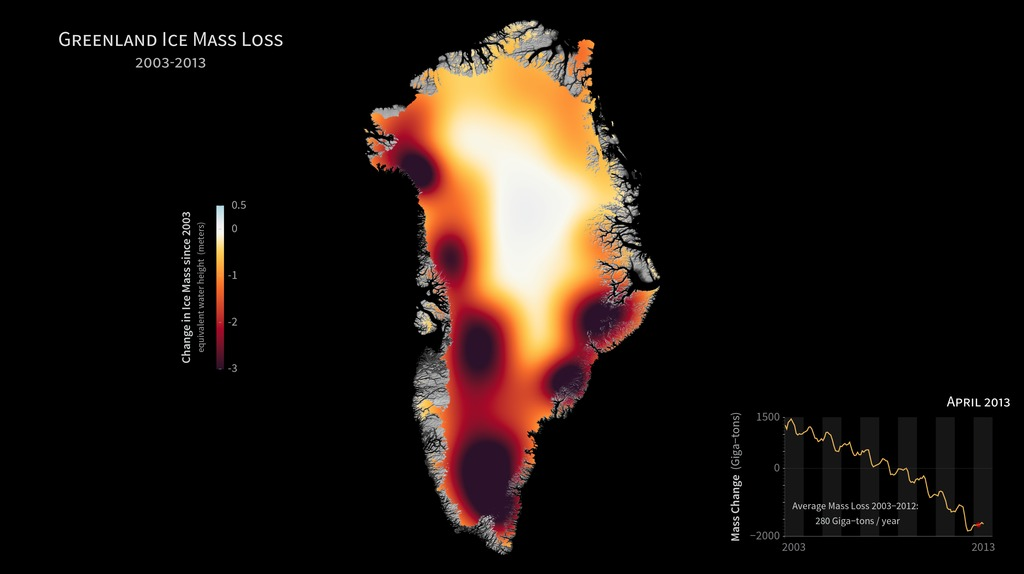
\includegraphics[width=12cm]{grace_greenland_2004_2012_still_print} \\
  \end{figure}
\end{frame}


\begin{frame}[plain]
    \begin{itemize}
    \item ice discharge to the ocean mostly through 200+ ``outlet glaciers''
    \item outlet glaciers are fast flows ($>$200\,m/yr), controlled by bedrock geometry, terminating in narrow fjords ($<$10\,km wide)
    \end{itemize}
    \begin{center}
      \includegraphics[width=9.5cm]{jako-front-positions}
    \end{center}
\end{frame}
 

\begin{frame}[plain]

\phantom{foo}

flow speeds vary over several orders of magnitude

\begin{itemize}
\item over distances of a few kilometers
\end{itemize}

\vspace{-5mm}
  \begin{columns}
    \column[c]{5.5cm}
    \begin{figure}
      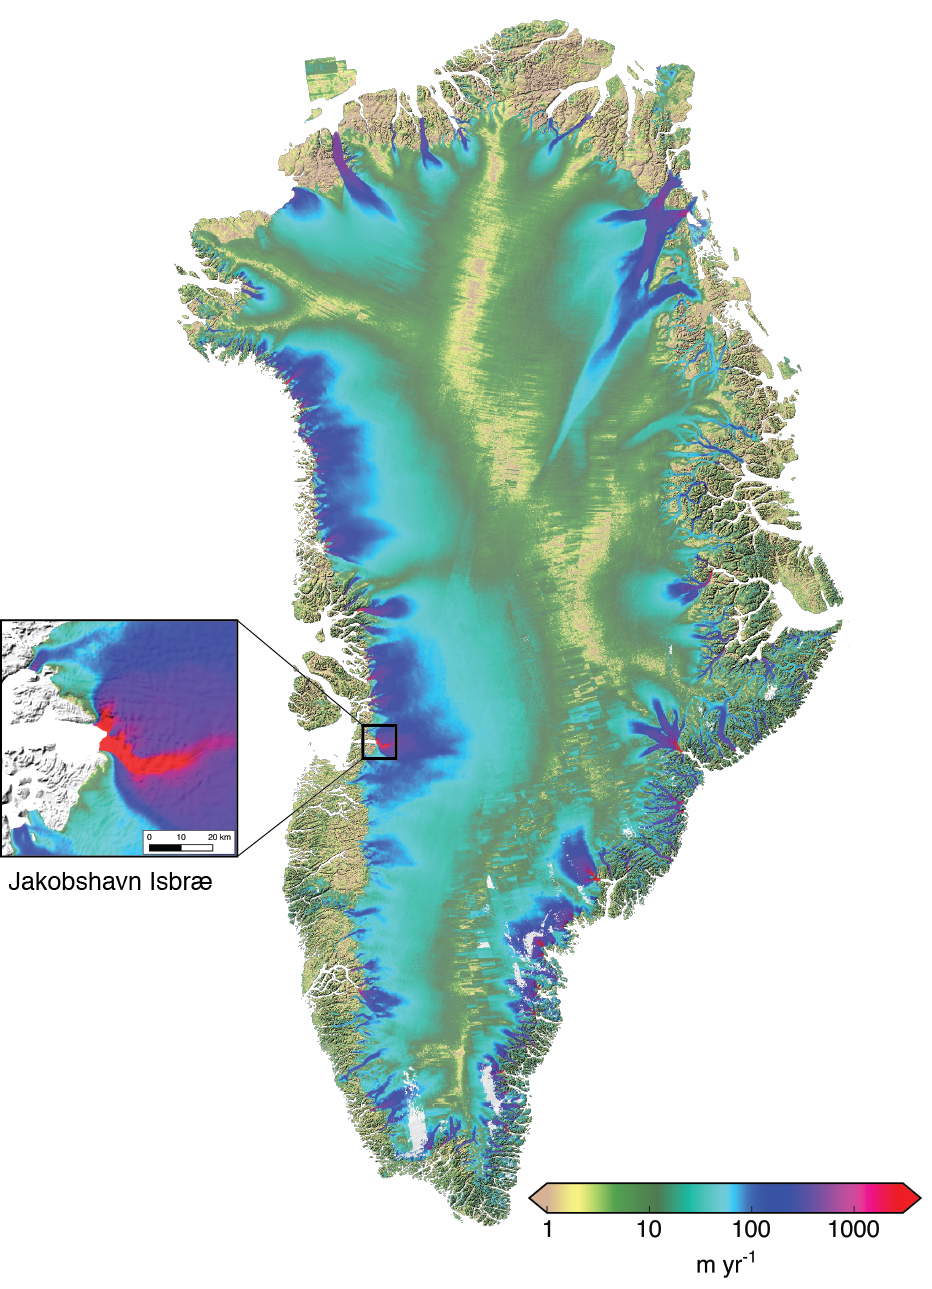
\includegraphics[width=\textwidth]{greenland-obs-overview}
    \end{figure}
    \column[c]{6cm}
    Jakobshavn Isbr{\ae}:
    
    \medskip
    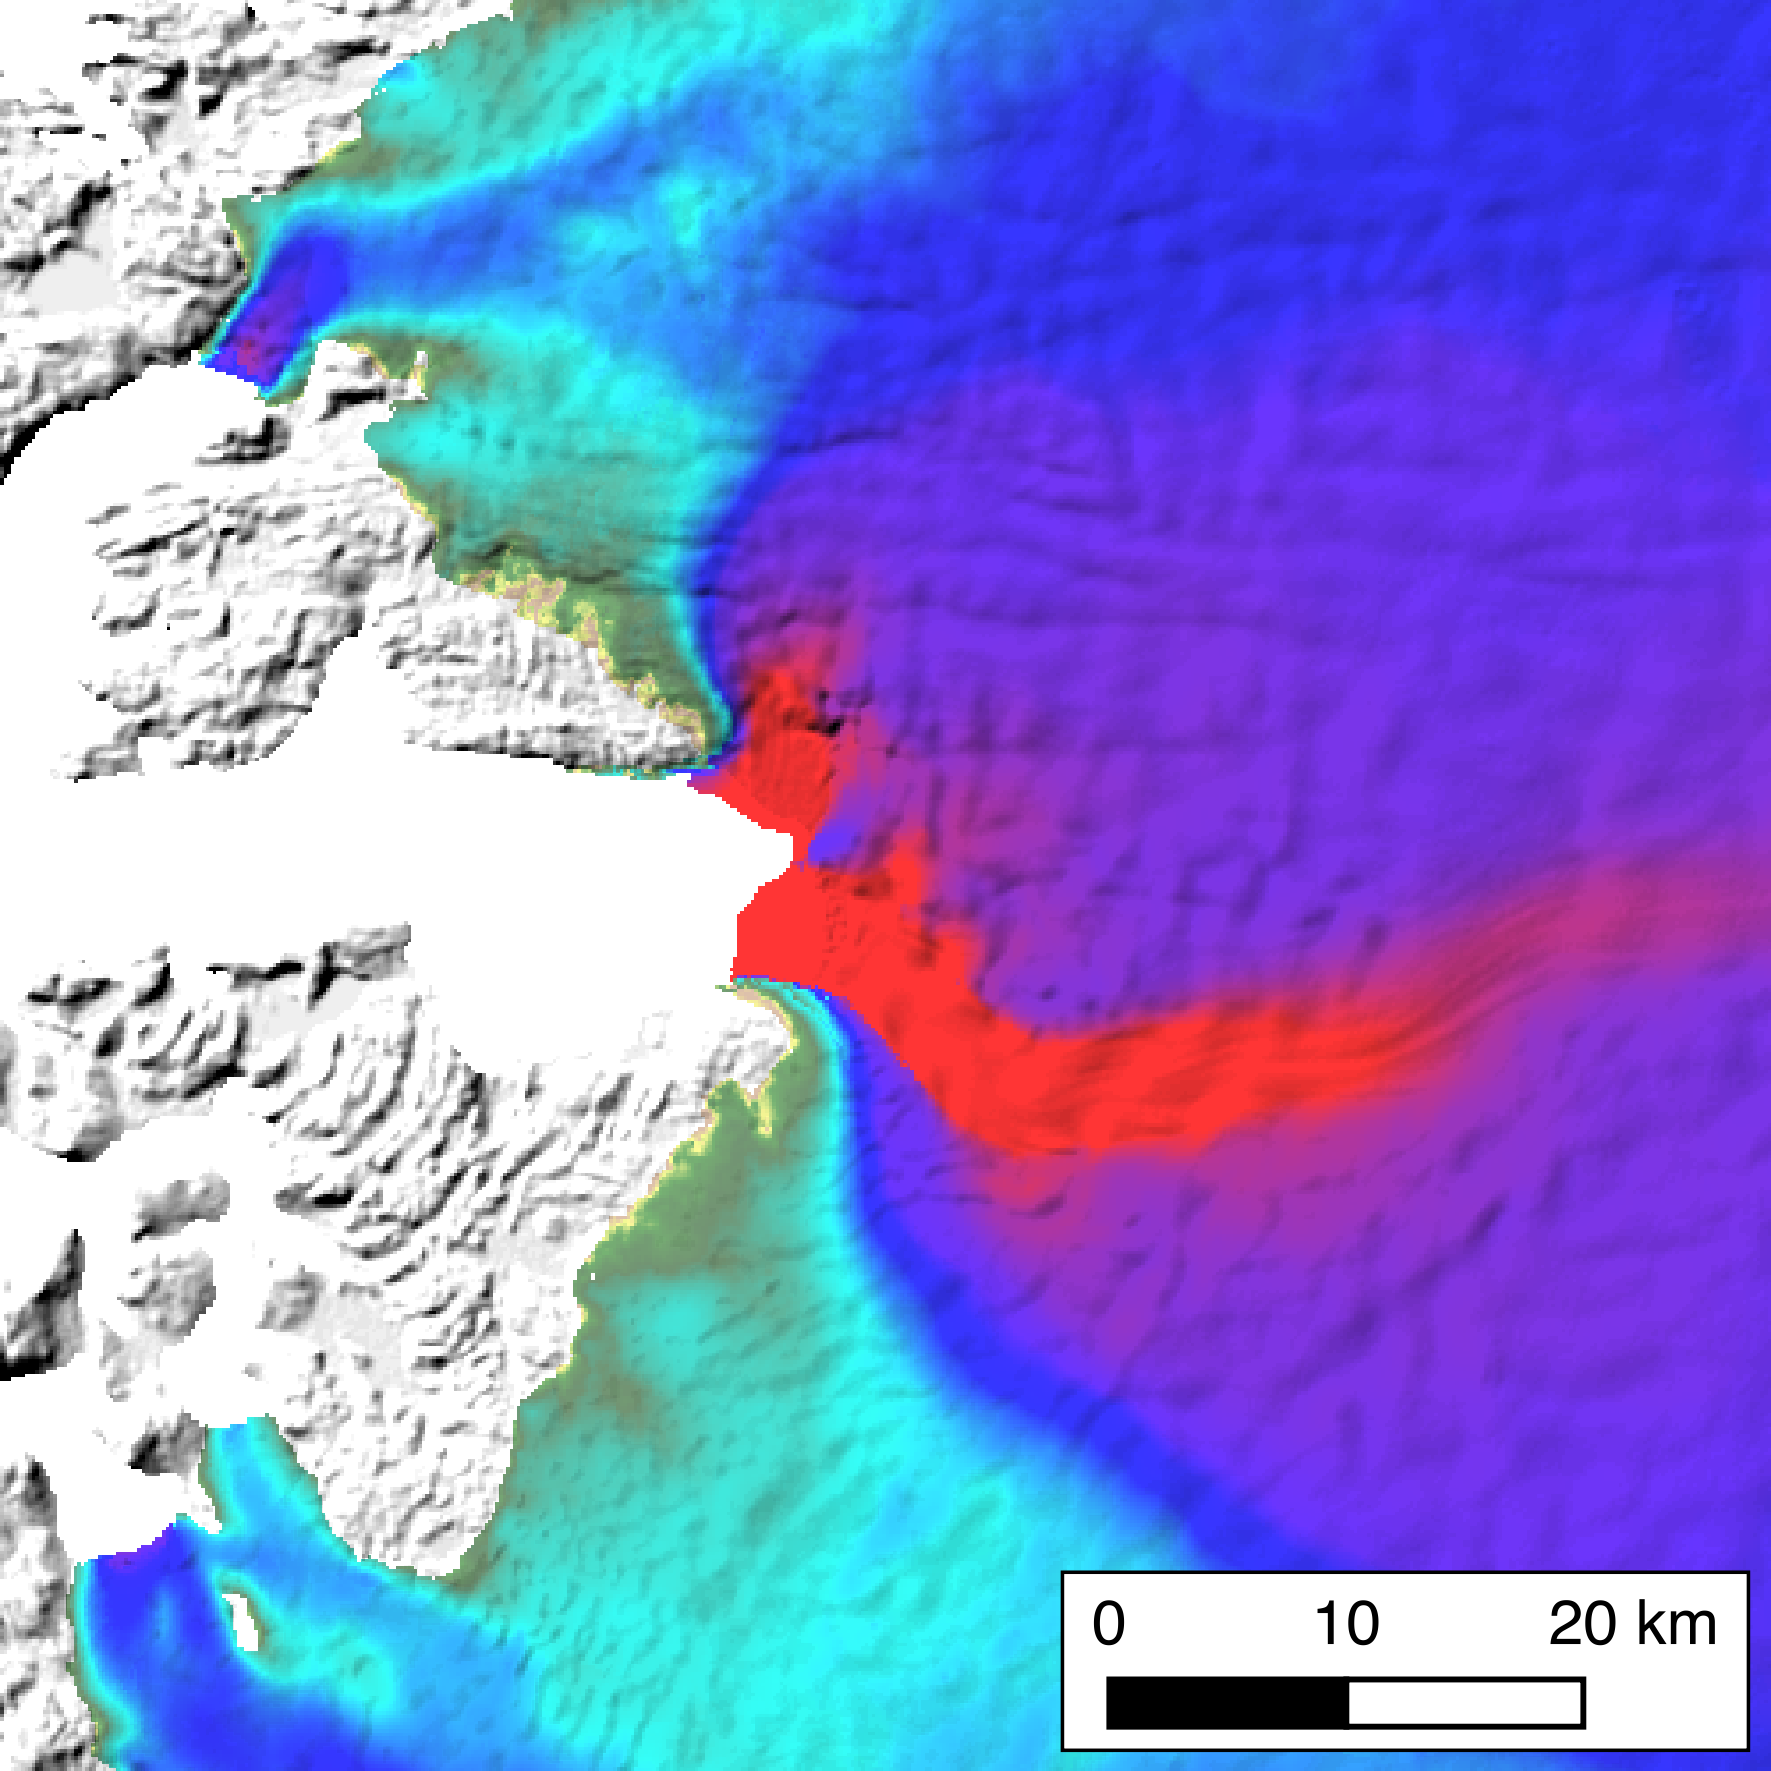
\includegraphics[width=\textwidth]{jakobshavn-obs-nogate}
  \end{columns}
\end{frame}


\begin{frame}[plain]

\begin{itemize}
\item modeling challenges in explaining variability of outlet glaciers:
      \begin{itemize}
      \item[$\circ$] \emph{resolution}:  must be high enough to resolve fjords
      \item[$\circ$] \emph{geometric data}: ice thickness is key to flow speed
      \end{itemize}
\item result: until recently, models failed to capture outlet glaciers
\end{itemize}

\bigskip

  \begin{columns}
    \column[c]{5cm}
    \emph{observed}

\medskip
    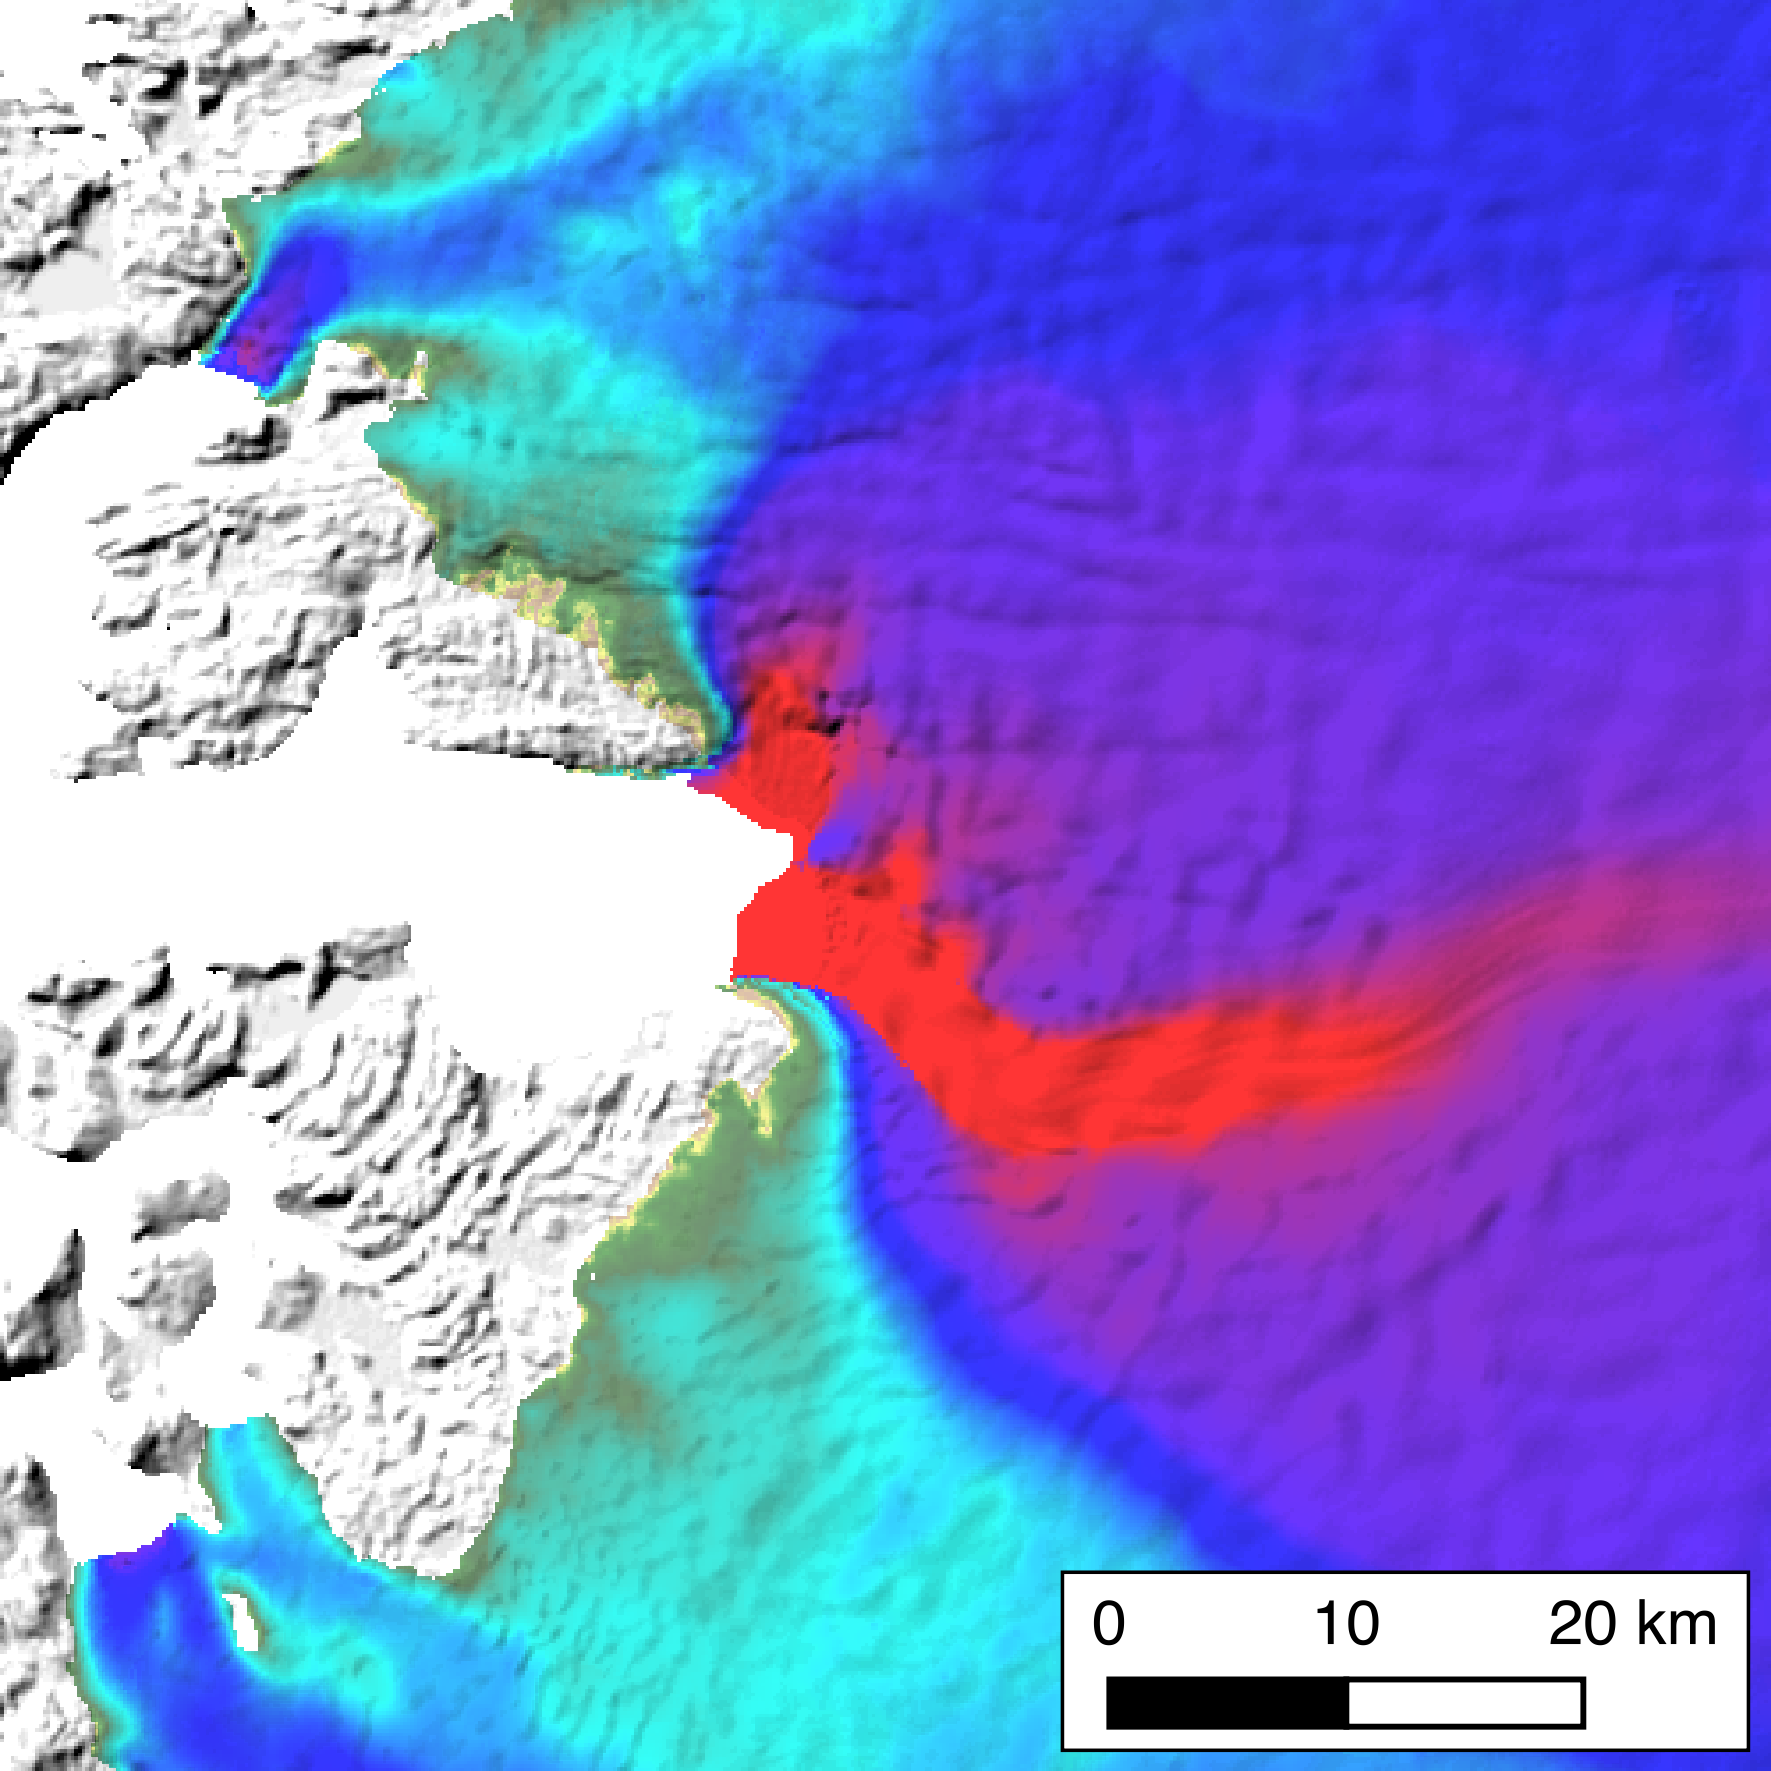
\includegraphics[width=\textwidth]{jakobshavn-obs-nogate}
    \column[c]{5cm}
    \emph{simulated circa 2009}

\medskip
    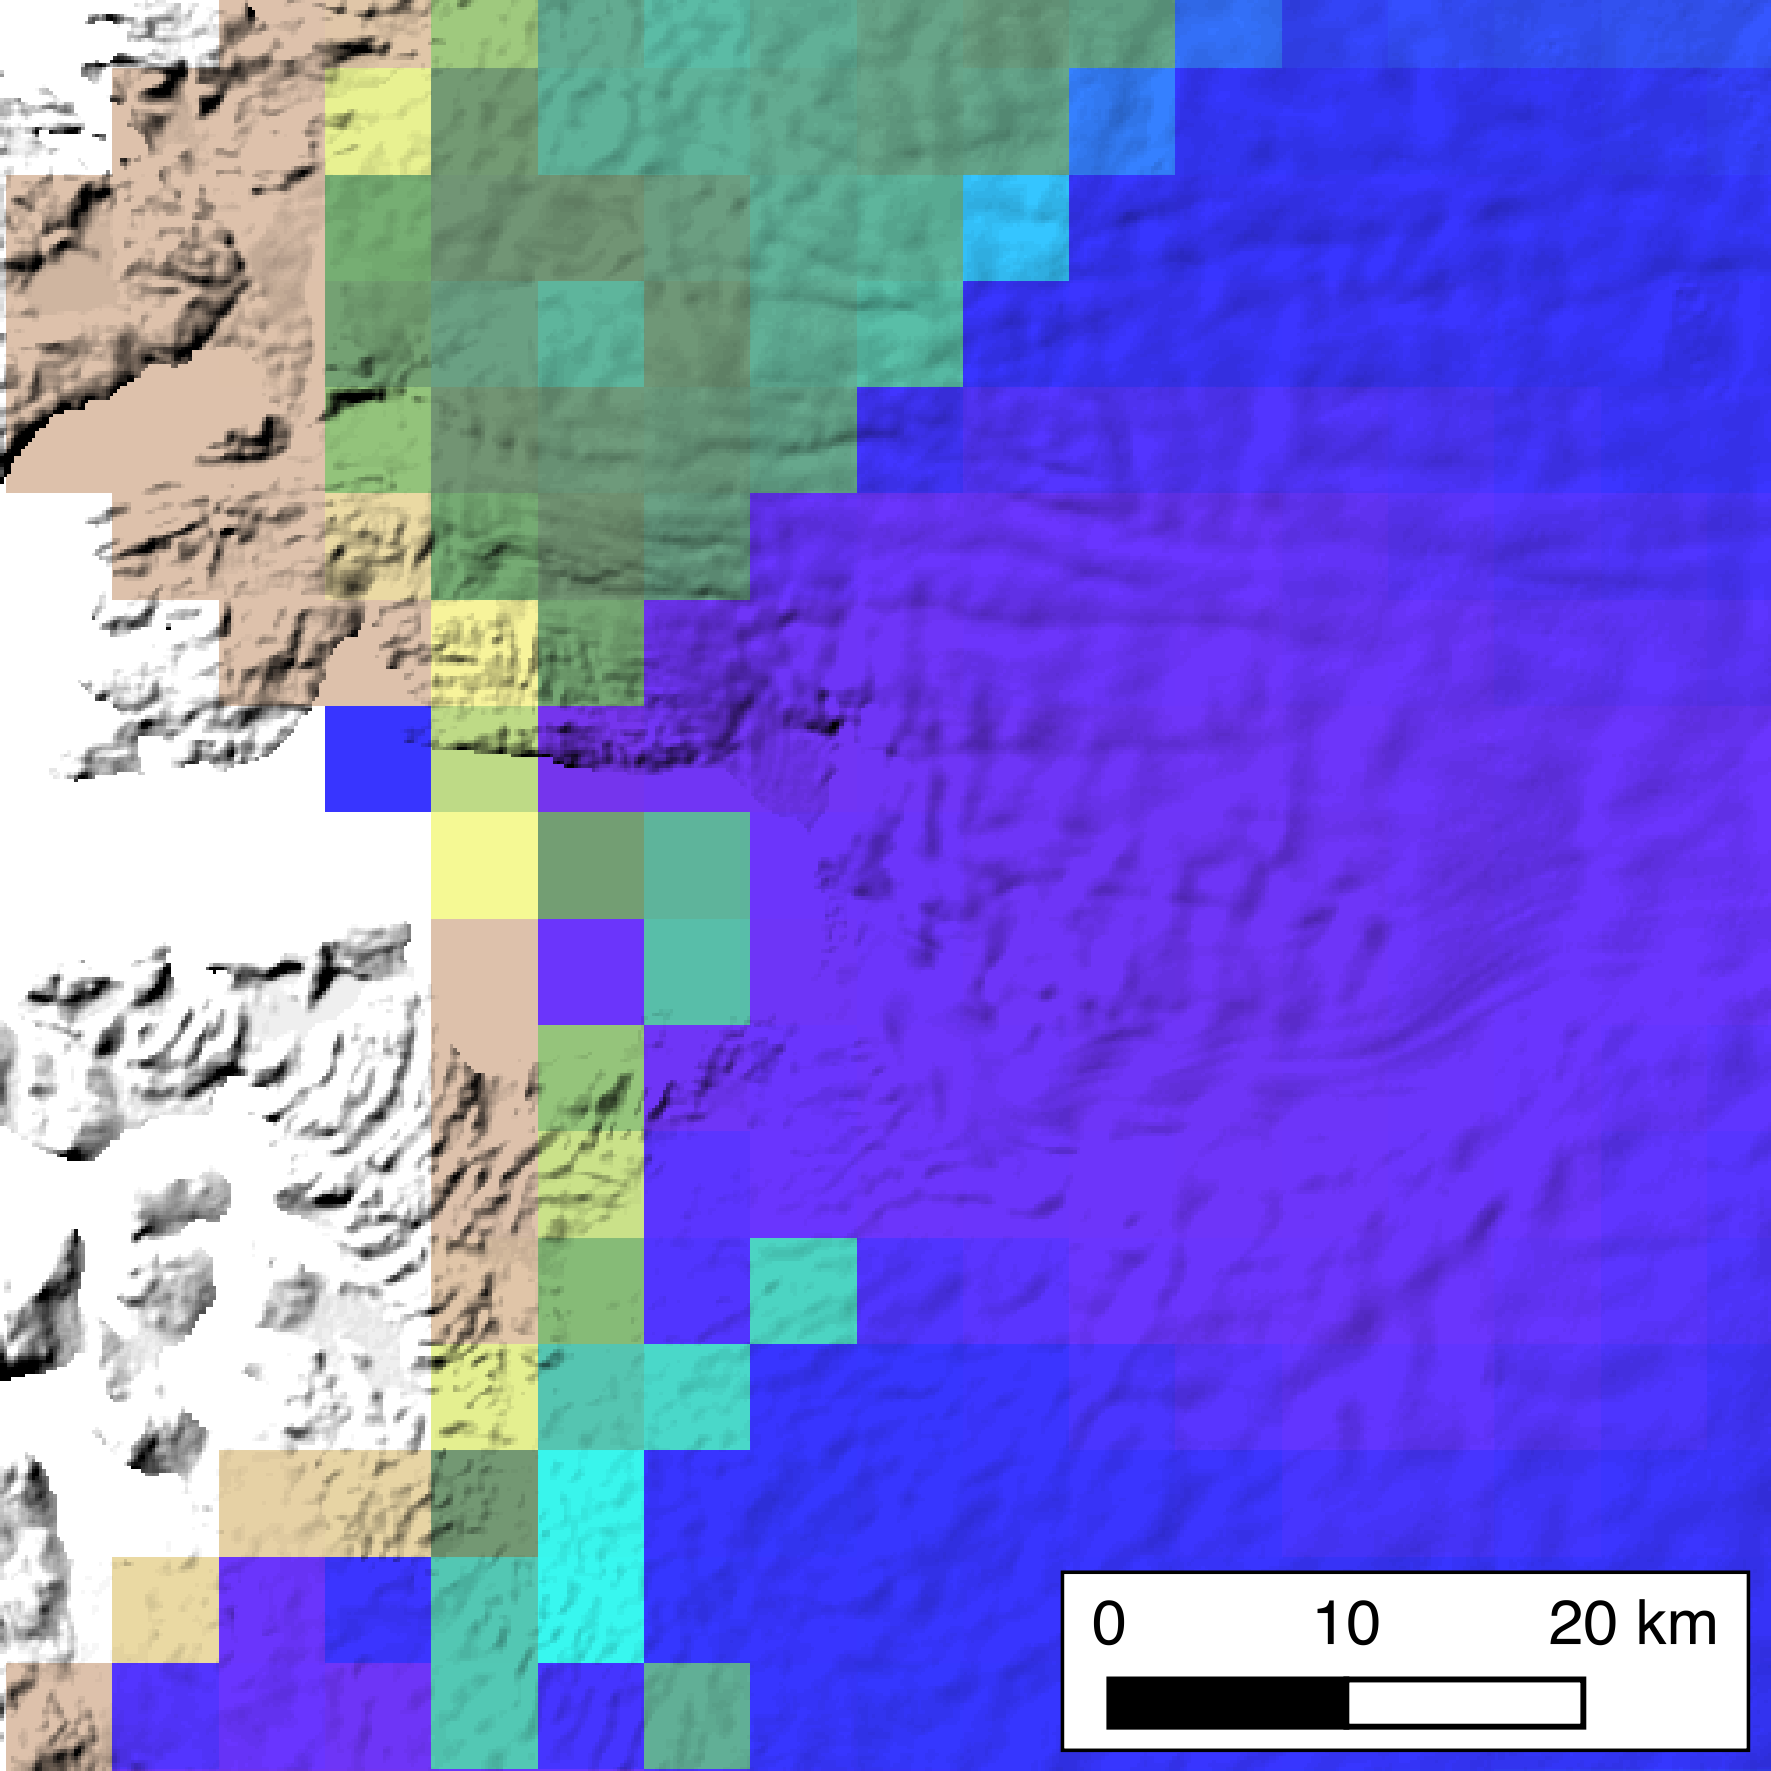
\includegraphics[width=\textwidth]{jakobshavn-speed-exp-4500m-ba01}
  \end{columns}
\end{frame}


\begin{frame}[plain]

\phantom{foo}

recent progress due to:

\begin{itemize}
\item model improvements (parallelism, better physics, etc)
\item many NASA airplane-based ice-penetrating-radar flights
\item improved map of bedrock under ice (below)
\end{itemize}

  \begin{figure}
    \small{Bamber (2001) \hspace{7em} Morlighem (2014)}
    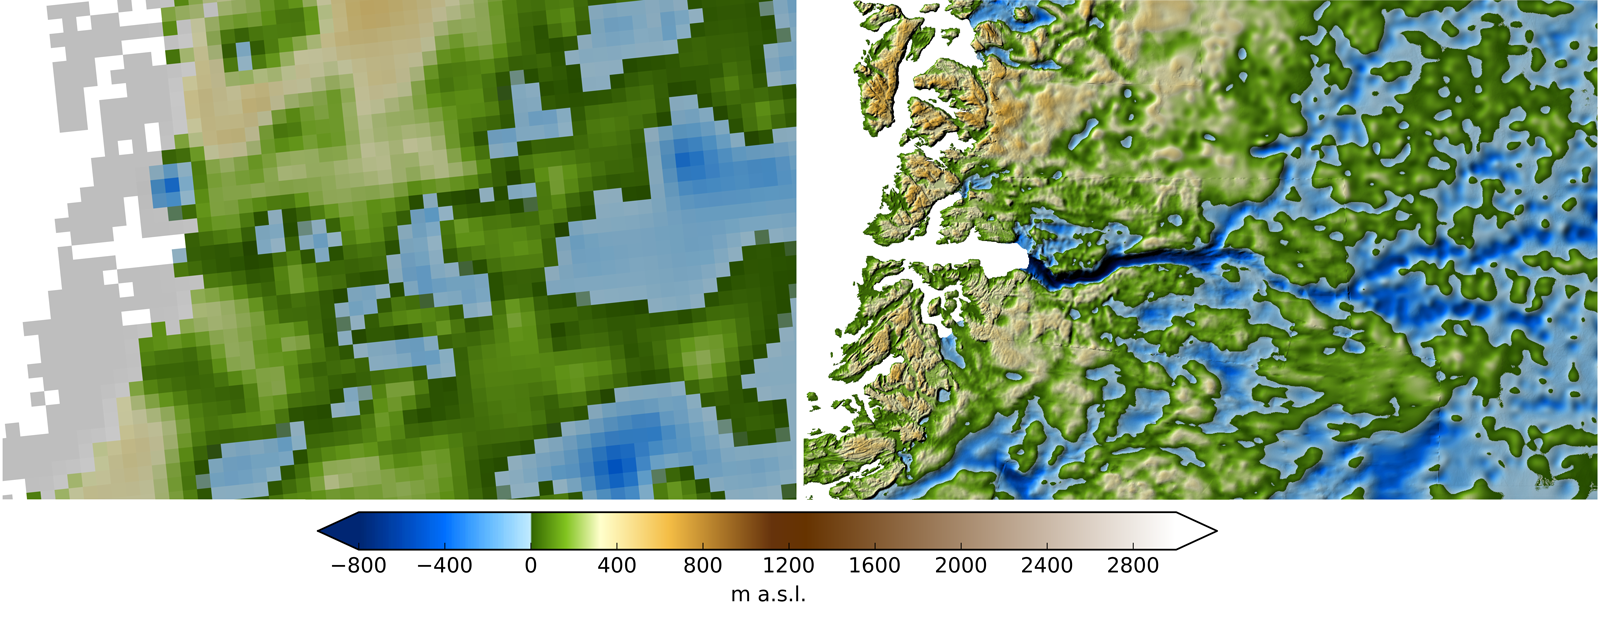
\includegraphics[width=12cm]{jako_bed}
 \end{figure}
\end{frame}


\setbeamertemplate{background canvas}
{
%
}


\begin{frame}{Parallel Ice Sheet Model (PISM)}
  \begin{itemize}
  \item open-source, fully-parallel from start in 2006
  \item primary development at UAF, with global user base
  \item $>$100k lines of code; mostly C++
  \item sustained NASA support \tiny (NAG5-11371, NNX09AJ38C, NNX13AM16G, NNX13AK27G)
  \end{itemize}
  \begin{columns}
    \column[c]{4.75cm}
    \begin{figure}
      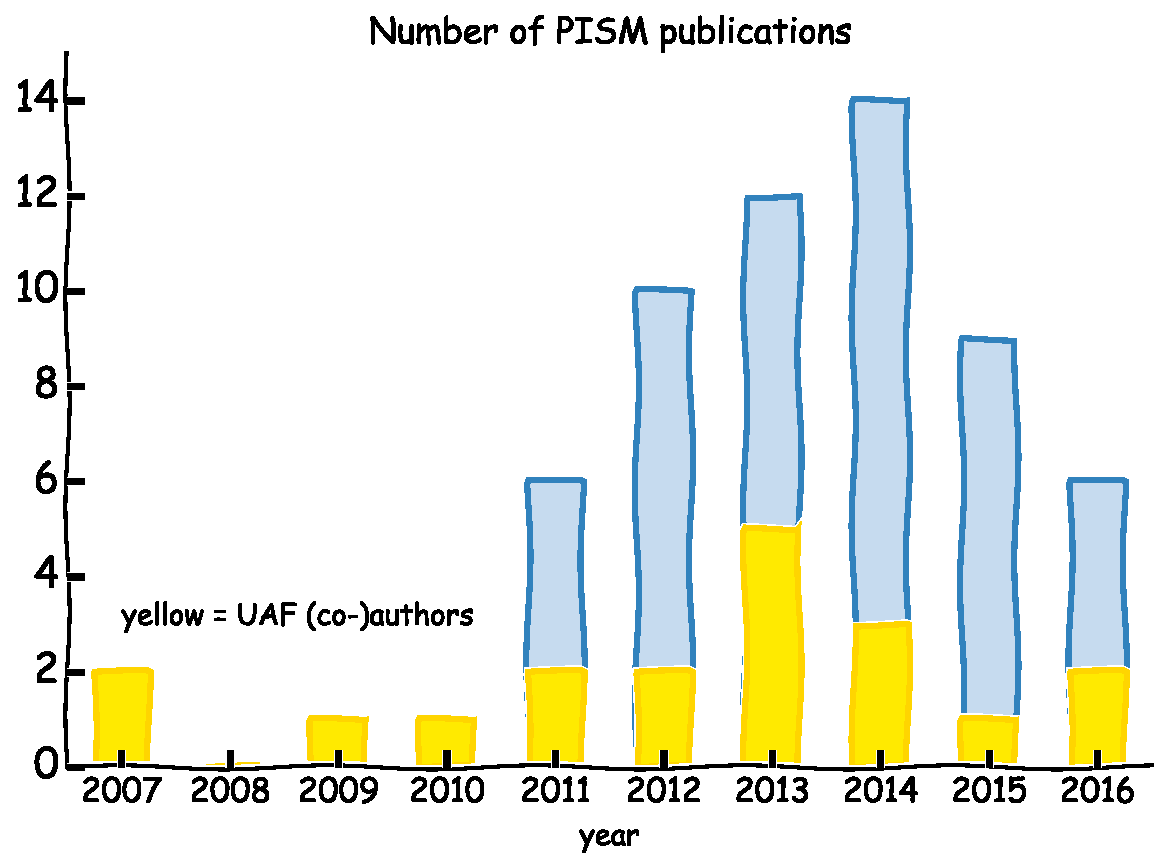
\includegraphics[width=\textwidth]{pism-uaf-publications}
    \end{figure}
    \column[c]{6.25cm}
    \includegraphics<1>[width=\textwidth]{pism-users}
  \end{columns}
\end{frame}


\begin{frame}{computational aspects}
  
  \begin{itemize}
  \item resolving outlet glacier flow requires horizontal grid resolutions $<$1\,km
       \begin{itemize}
       \item[$\circ$] ideally $<$500\,m
       \item[$\circ$] on current UAF HPC resources, a 100 year long simulation at 600\,m resolution takes $\sim$ 120 wall clock hours on 500 cores
       \item[$\circ$] only selected simulations can be run at the required resolutions
       \end{itemize}
  \item PISM simulations benefit from
    \begin{itemize}
    \item \emph{more nodes}: higher resolutions
    \item \emph{faster CPUs}: reduced integration times for long simulations
    \end{itemize}
\end{itemize}
\end{frame}


\begin{frame}{access to local HPC resources is crucial}

    \begin{itemize}
    \item the UAF PISM team does
       \begin{itemize}
       \item[$\circ$] fast, iterative code development and testing
       \item[$\circ$] constant scaling and performance analysis during development
       \end{itemize}    
    \item result is cutting-edge science
       \begin{itemize}
       \item[$\circ$] 12 PISM-using publications in \emph{Science, Nature, PNAS} journals
       \item[$\circ$] including new Greenland ice sheet results from UAF (below)
       \end{itemize}
    \end{itemize}

\begin{center}
    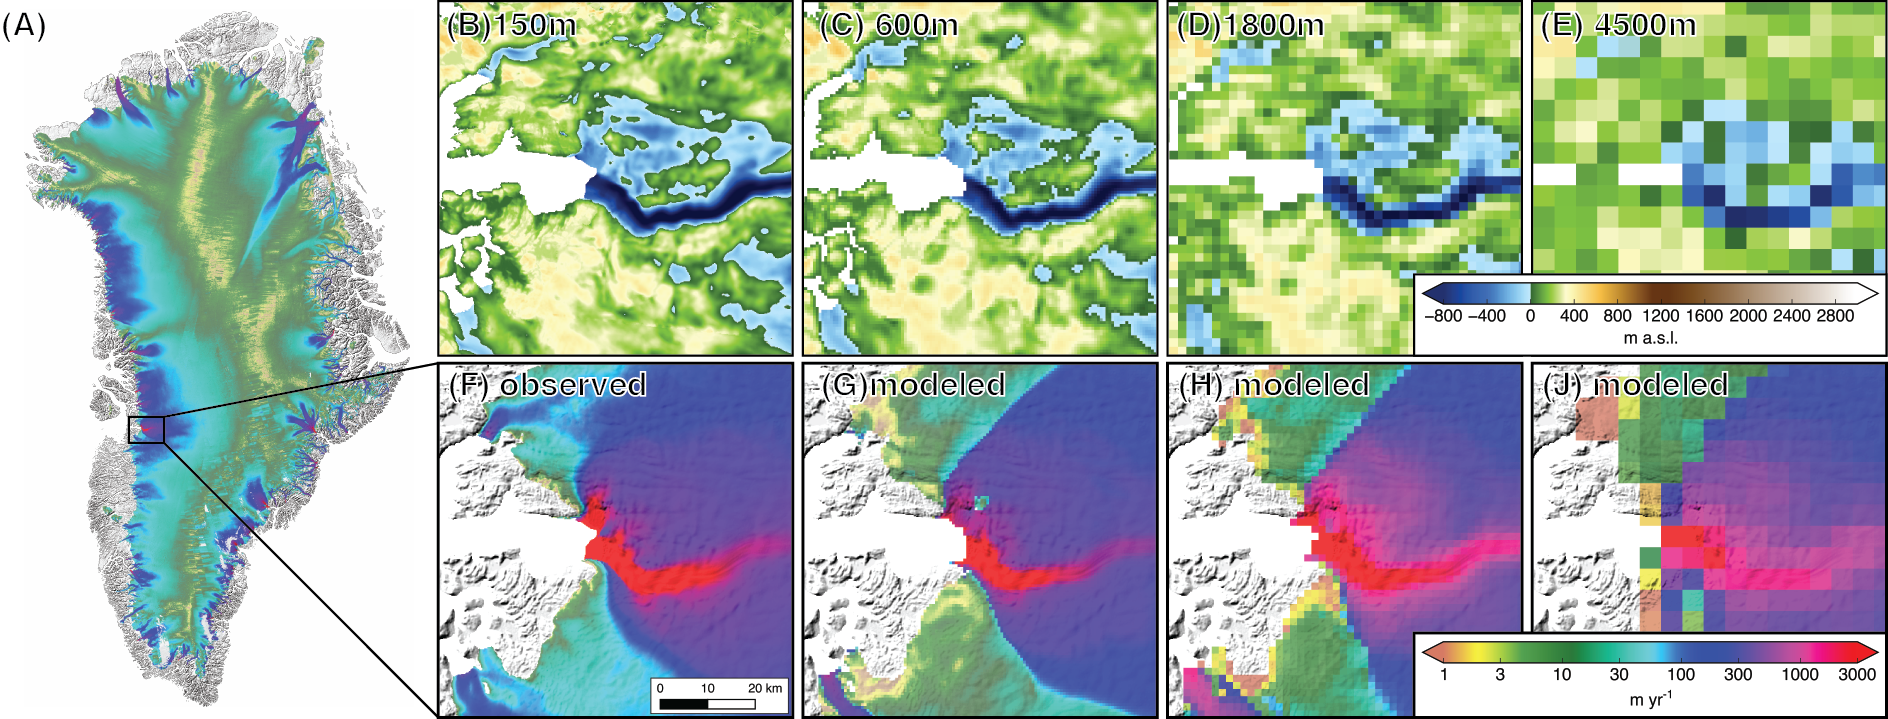
\includegraphics[width=0.8\textwidth]{jakobshavn-beds}
    \\ \hfill \scriptsize from Aschwanden, Fahnestock, \& Truffer, \emph{Nature Comm.} 2016
\end{center}
\end{frame}


\end{document}

